\section{Design of the Solution}
\label{sec:design}

This section presents the design of the system in the Unified Modeling Language (UML) \refUML{}.
This project wrote all UML diagrams in the Mermaid text notation \refMermaid{}.

\subsection{System Architecture}

Figure~\ref{fig:architecture} presents the four layers of the system.
Each layer depends only on the layers below it.
The presentation layer contains the three user interfaces.
The application layer offers the operations that these interfaces share.
The parsing and analysis layer turns netlist text into objects and runs simulations and analyses.
The domain model layer represents the circuit itself.

The browser version reuses the Java layers without a server.
The TeaVM compiler \refTeaVM{} translates the Java engine to JavaScript.
The class \texttt{WasmBridge} exports functions that accept netlist text and return JSON, and the page \texttt{index.html} calls these functions and draws the results.

\begin{figure}[H]
\centering
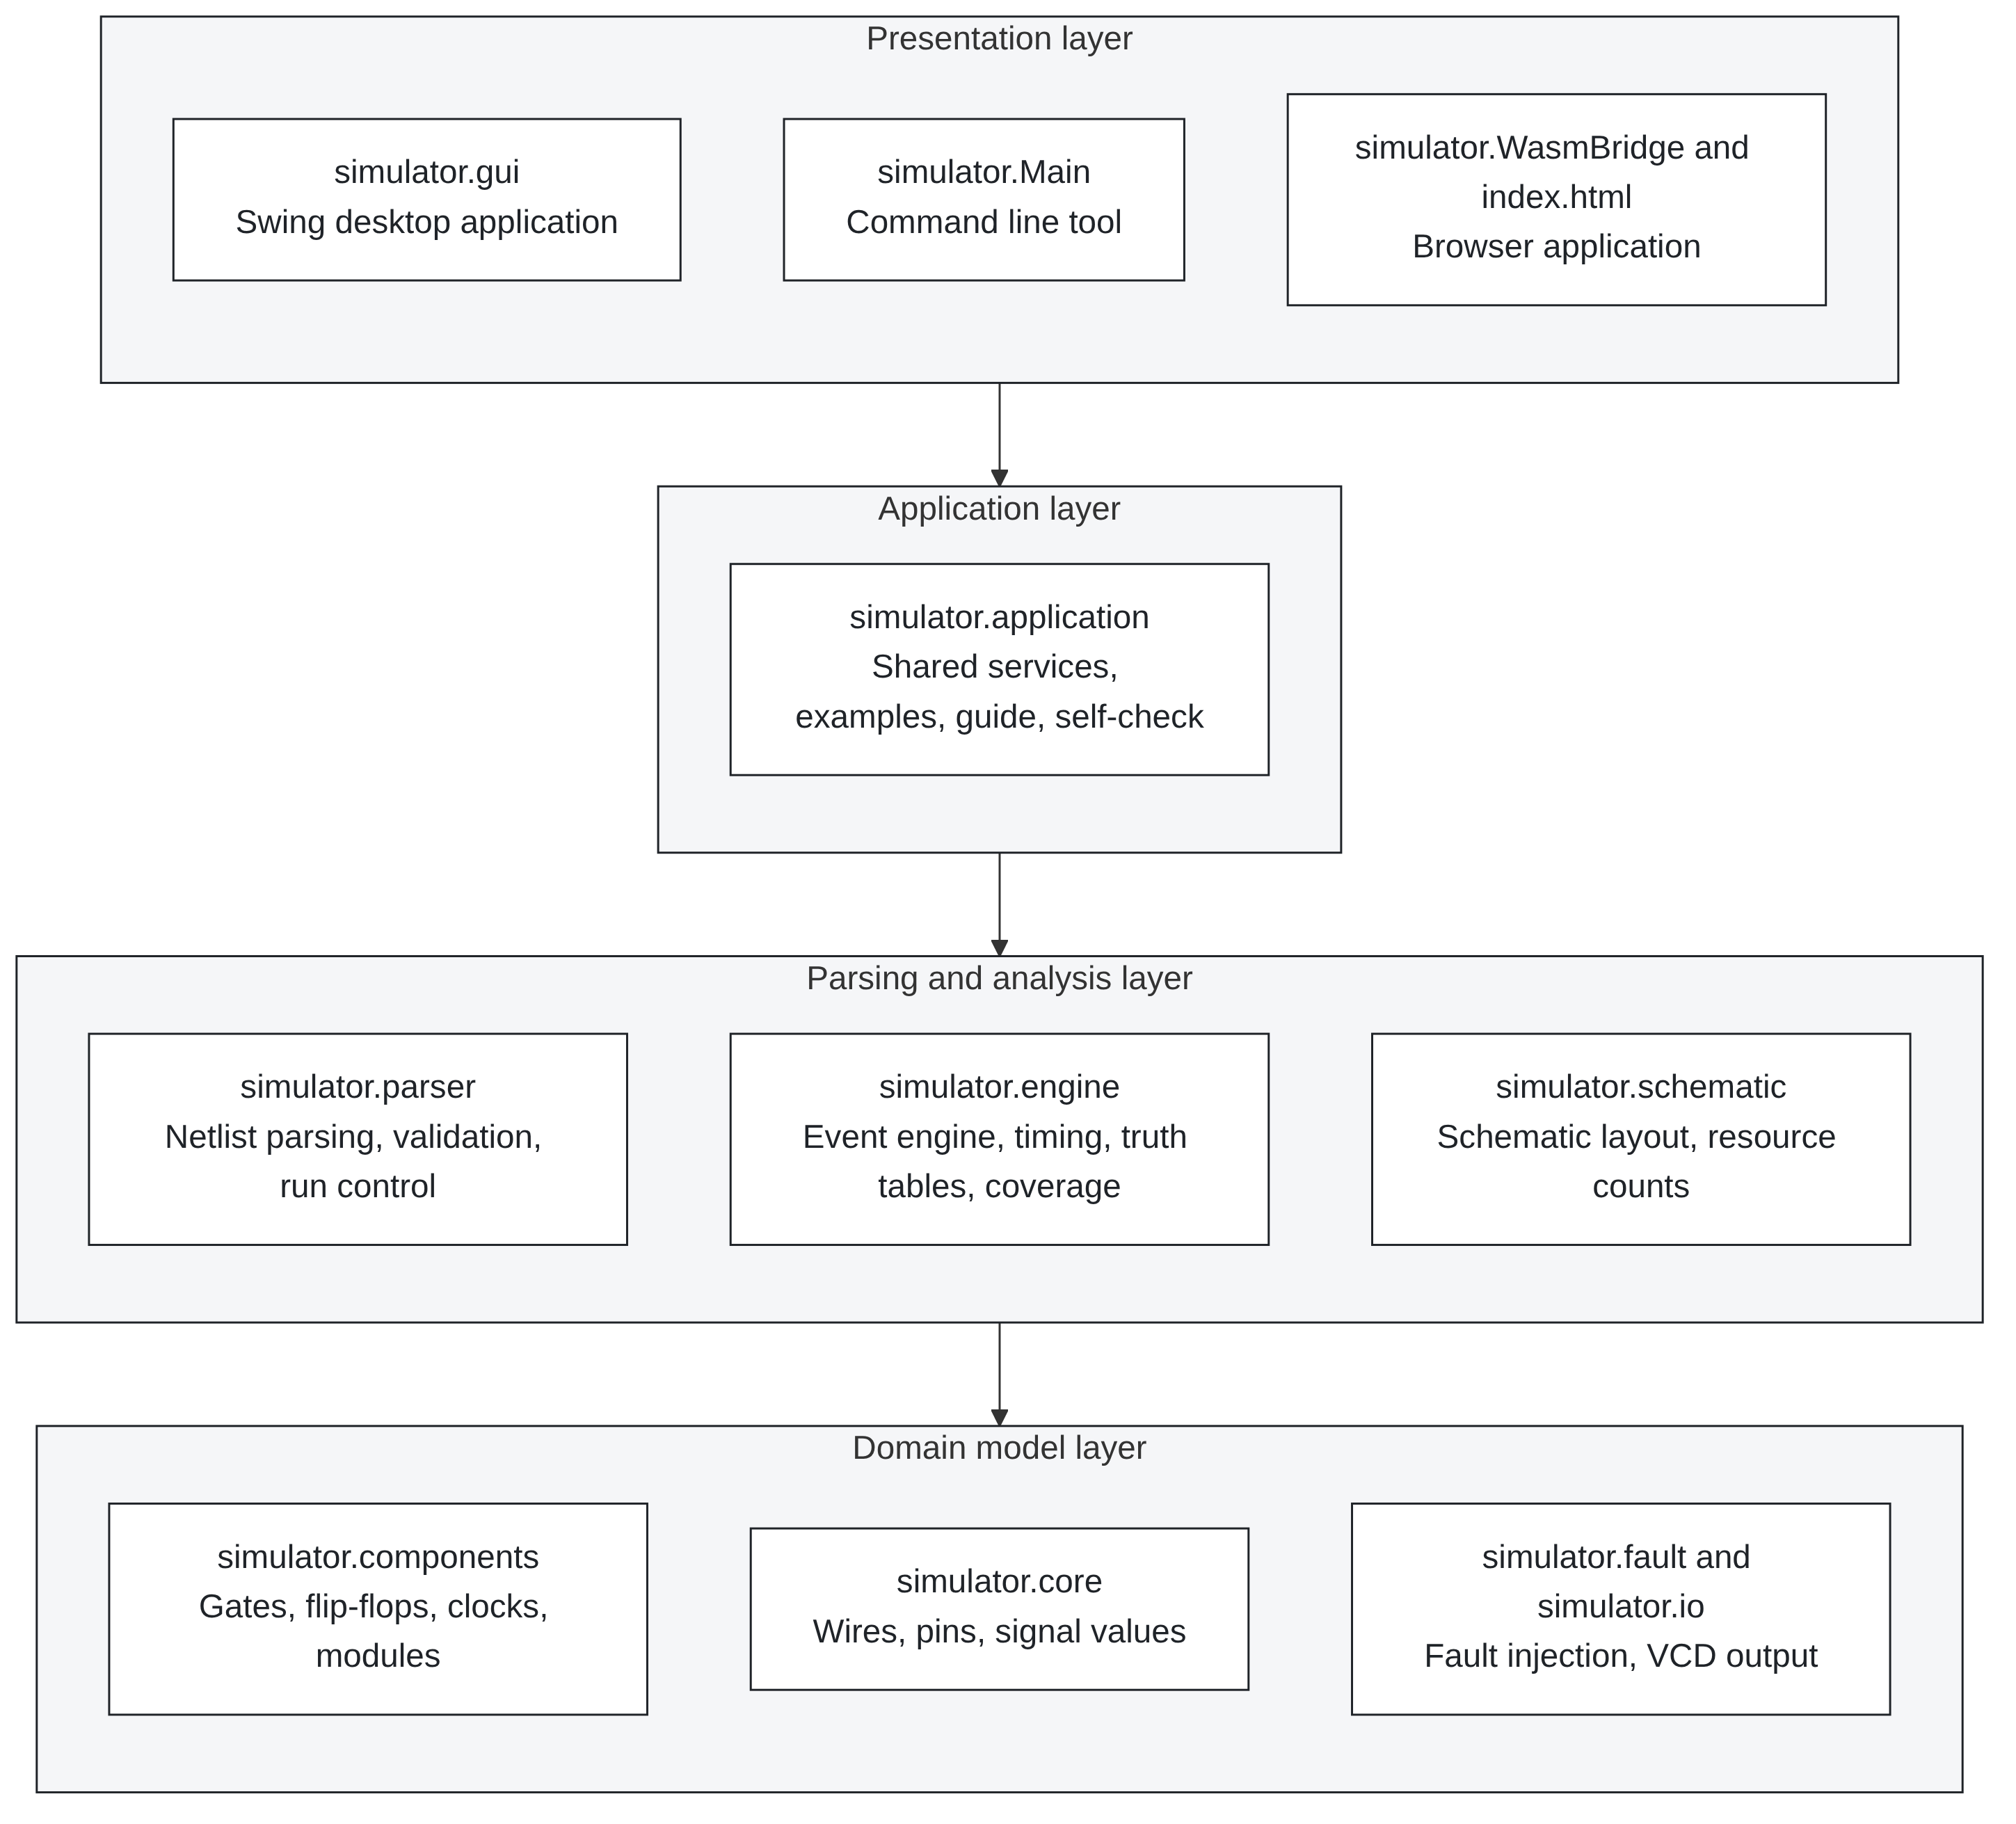
\includegraphics[width=0.9\textwidth]{architectureDiagram.png}
\caption{Layered architecture of the system}
\label{fig:architecture}
\end{figure}

\subsection{Class Model}

Figure~\ref{fig:classdomain} presents the domain model.
\texttt{DigitalComponent} is the abstract base class of every component and owns its pins.
\texttt{LogicGate} adds a propagation delay and schedules an event when its calculated output changes.
Each concrete gate implements only its own Boolean function.
The figure groups the seven simple gates into one box to save space.
A \texttt{Wire} connects output pins to input pins and resolves the values of its drivers into one value.

\begin{figure}[H]
\centering
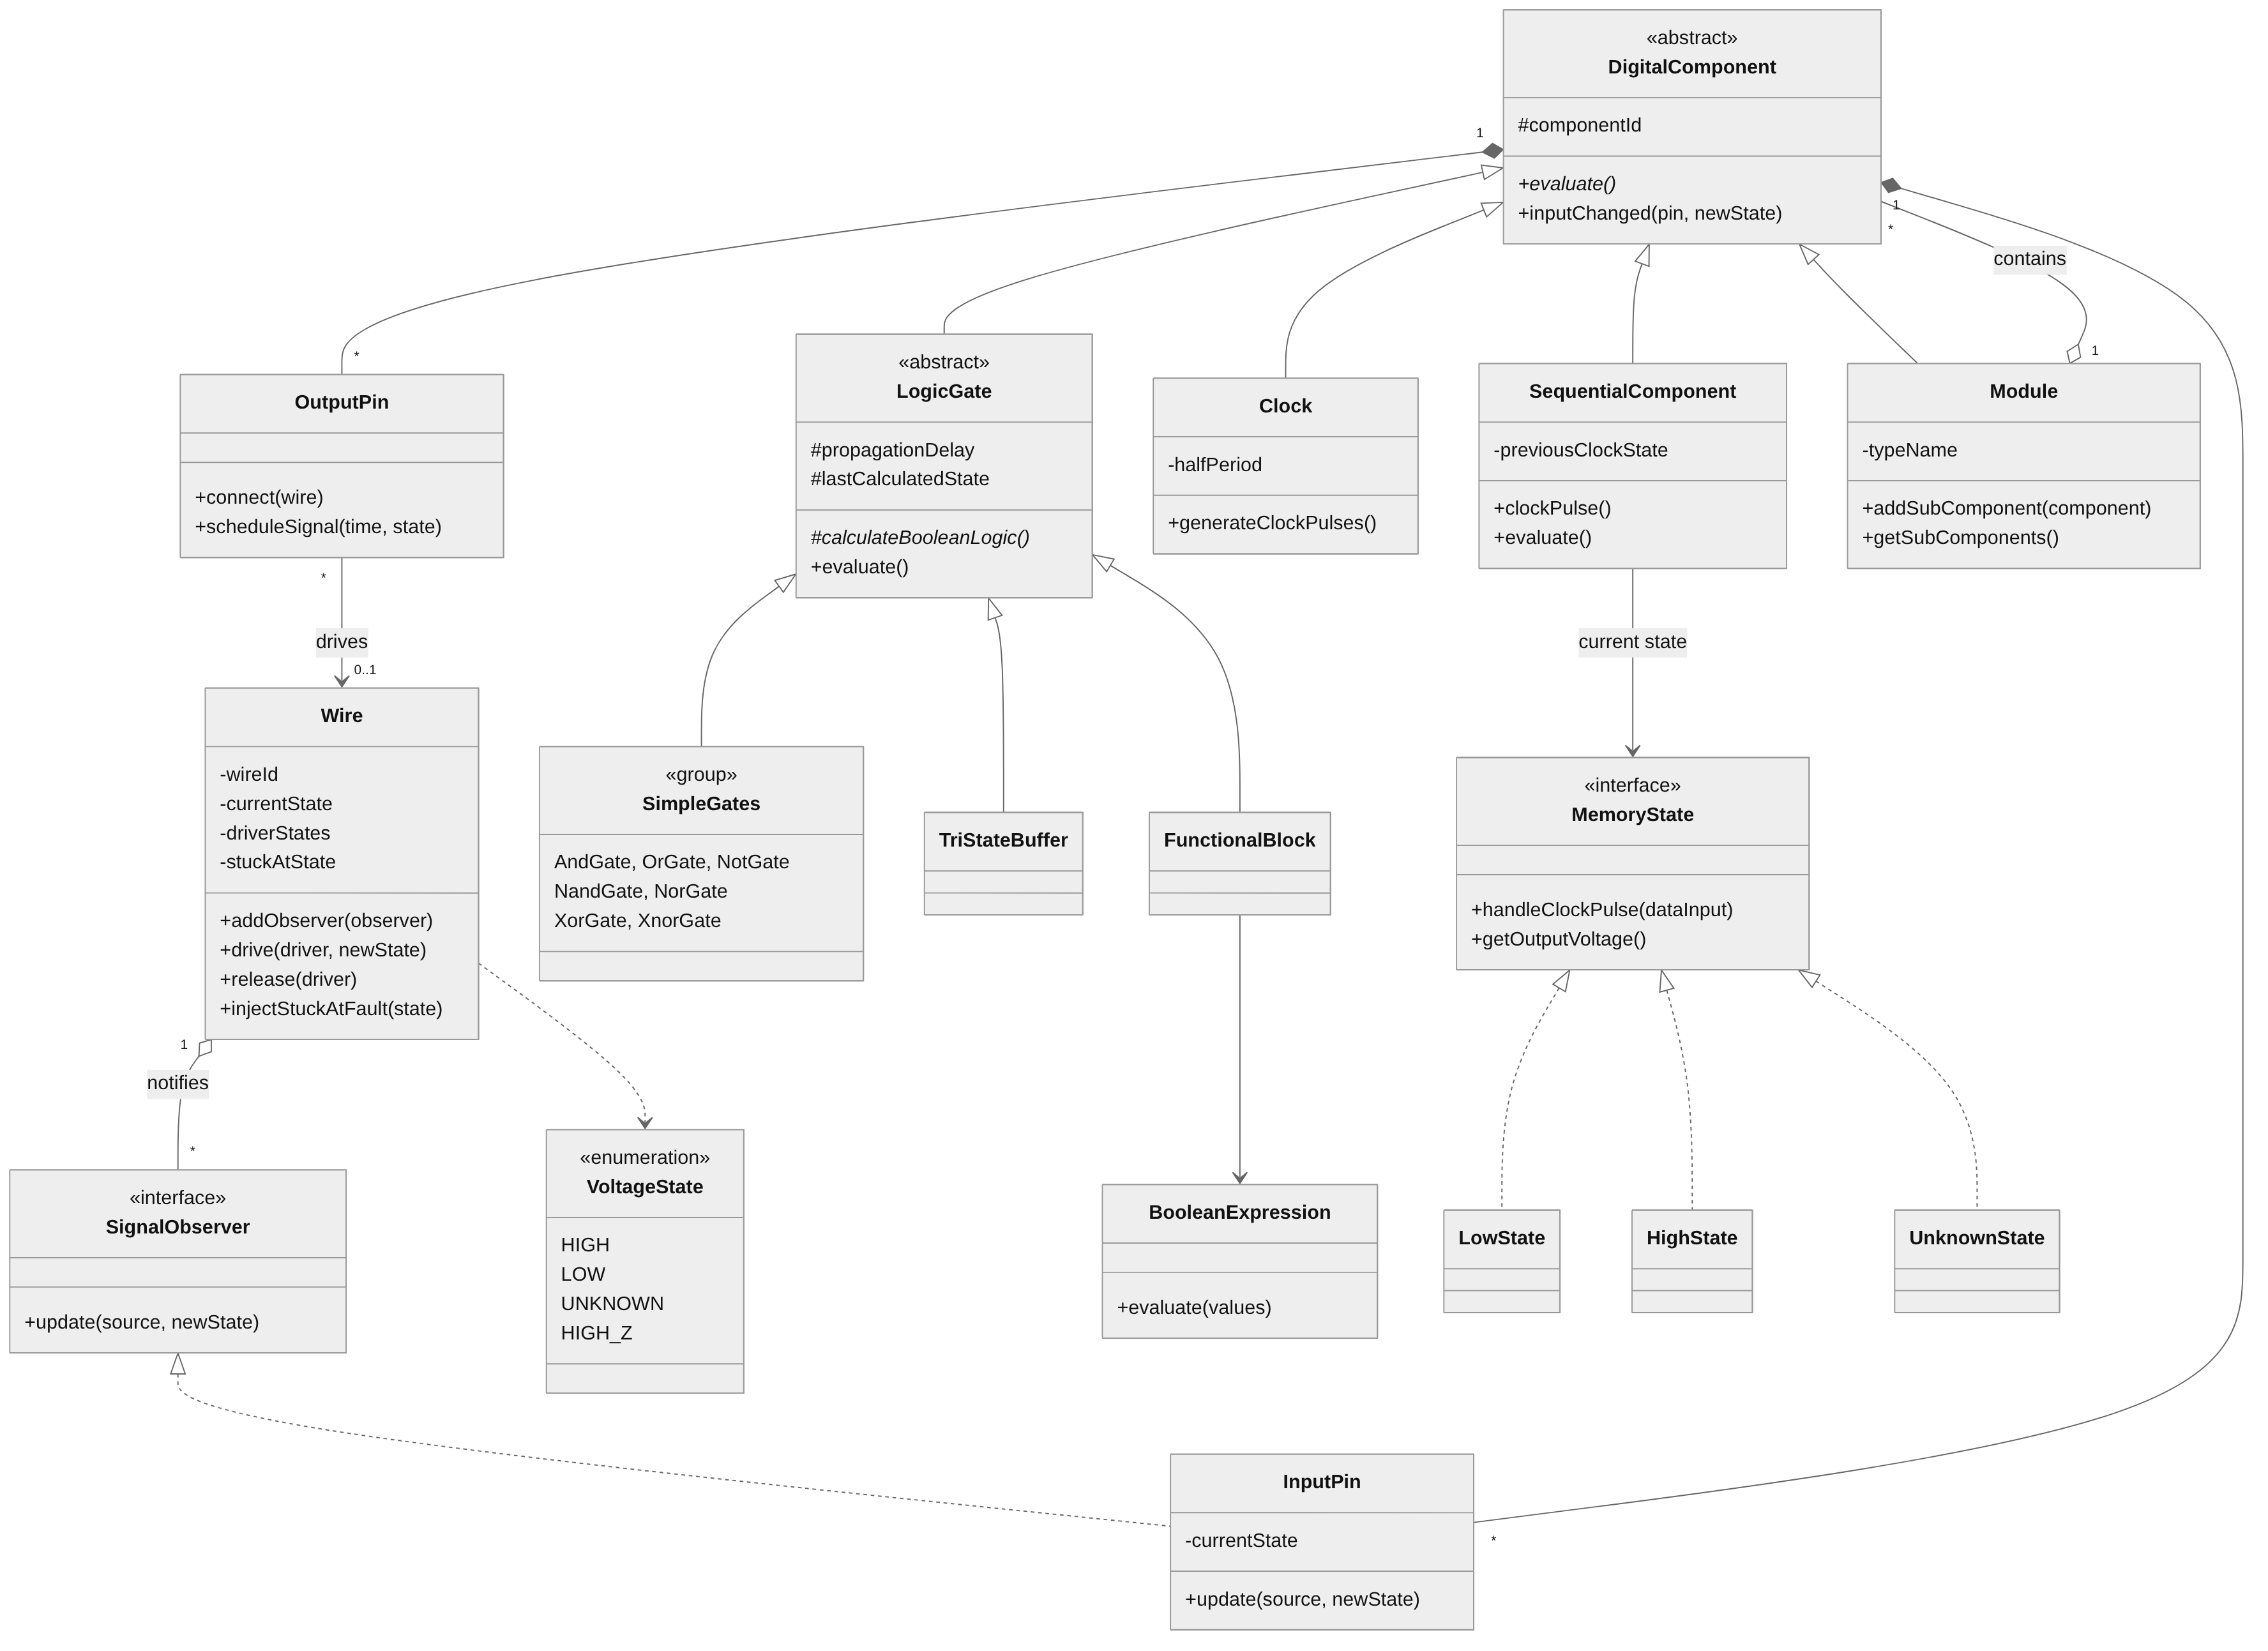
\includegraphics[width=\textwidth]{classDiagramDomain.png}
\caption{Class diagram of the domain model}
\label{fig:classdomain}
\end{figure}

Figure~\ref{fig:classengine} presents the parsing, engine, and analysis classes.
\texttt{SimulationRunner} coordinates a single simulation run.
\texttt{SimulationContext} owns the \texttt{EventEngine} and the assertions of that run.
The analysis classes create their own contexts, so their internal simulations remain separate from each other.

\begin{figure}[H]
\centering
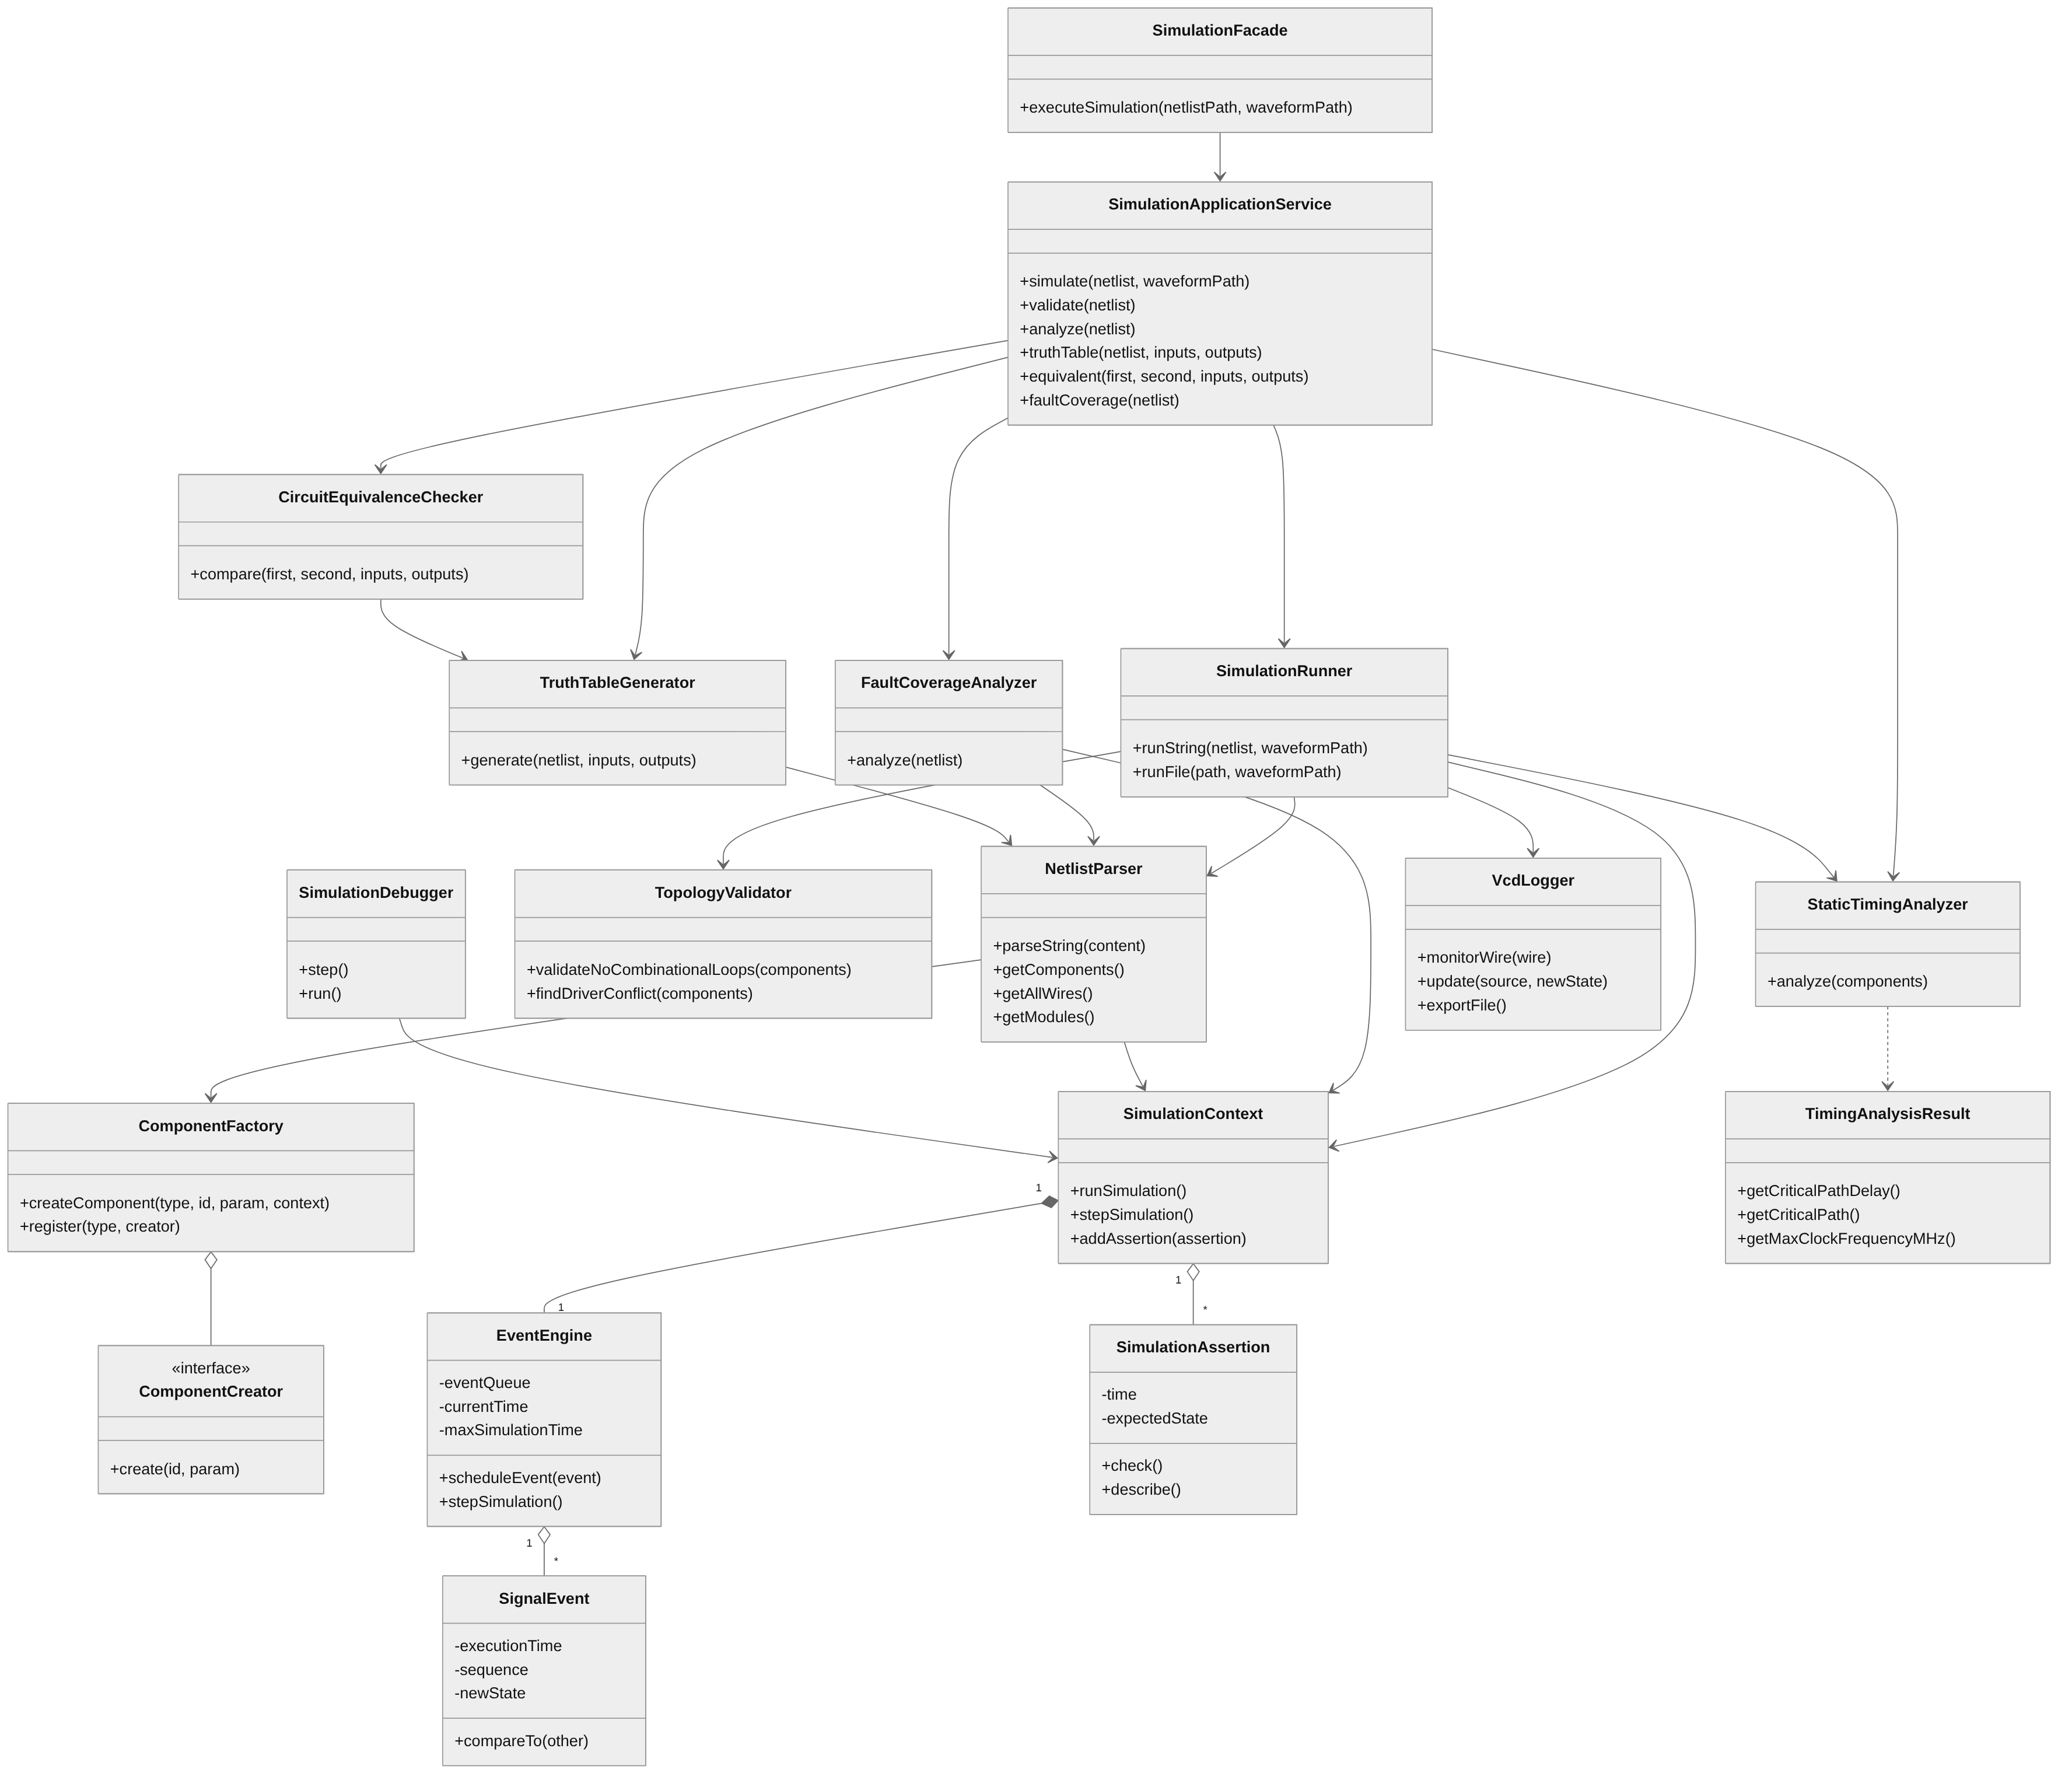
\includegraphics[width=\textwidth]{classDiagramEngine.png}
\caption{Class diagram of the parsing, engine, and analysis classes}
\label{fig:classengine}
\end{figure}

\subsection{Interaction Model}

Figure~\ref{fig:seqrun} presents the messages of one simulation run.
The user interface passes the netlist to the service, and \texttt{SimulationRunner} carries out the phases of the pipeline in order.

\begin{figure}[H]
\centering
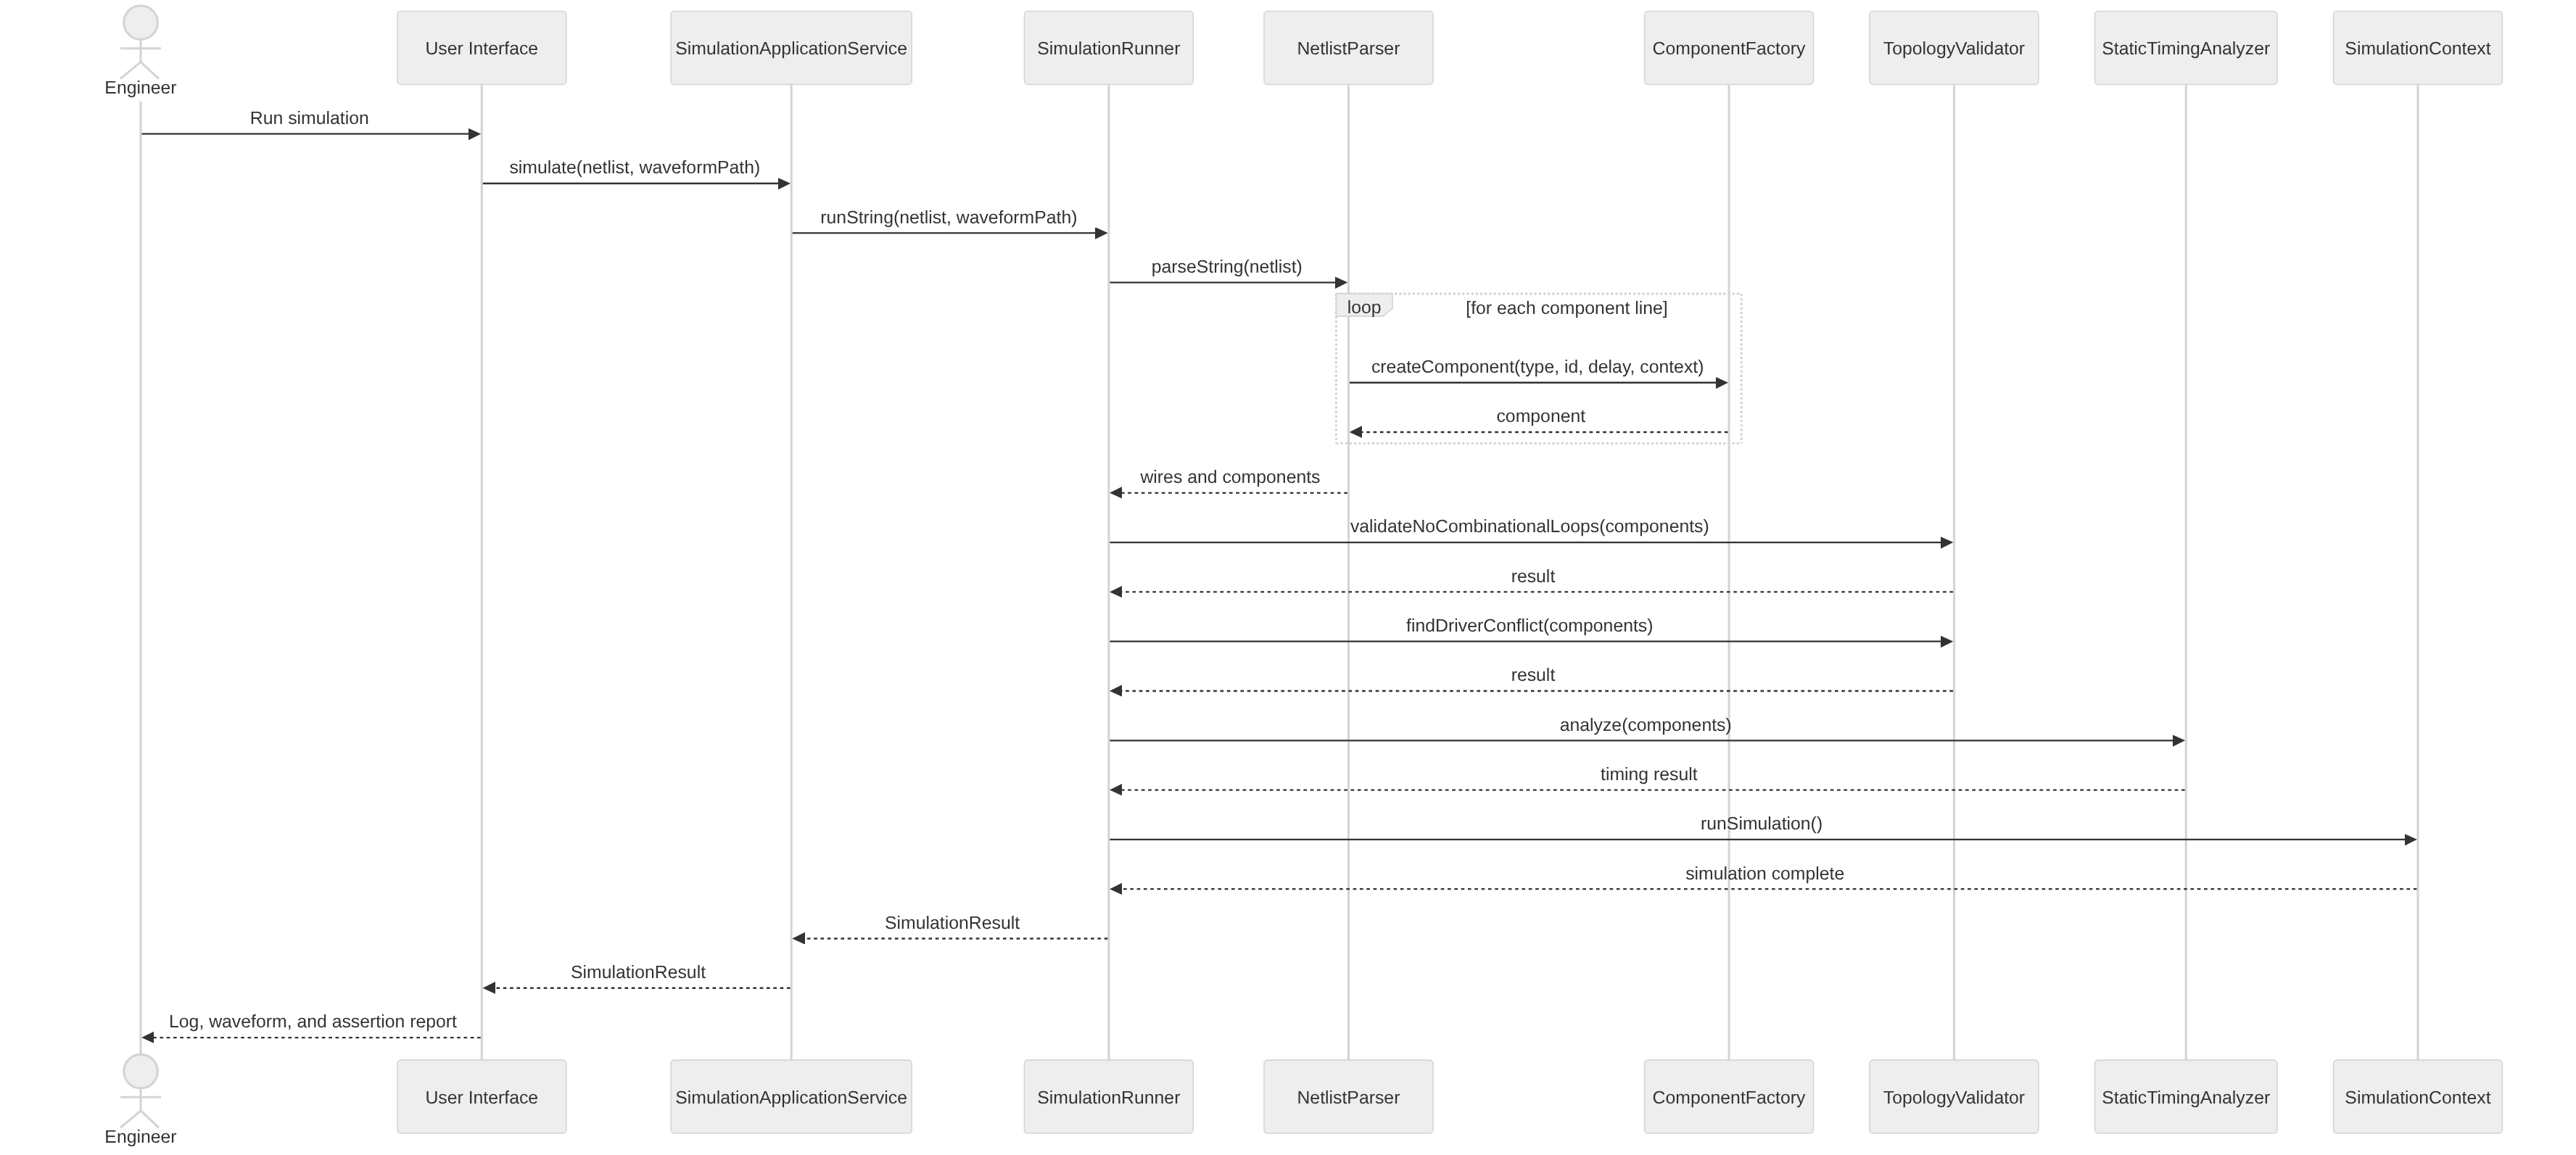
\includegraphics[width=\textwidth]{sequenceDiagramRun.png}
\caption{Sequence diagram of a simulation run}
\label{fig:seqrun}
\end{figure}

Figure~\ref{fig:seqevent} presents the processing of one event.
The queue orders events by time and then by creation order, so a given netlist always produces the same result.
A gate schedules a new event only when its calculated output changes.
The engine therefore avoids work for signals that have no effect.

\begin{figure}[H]
\centering
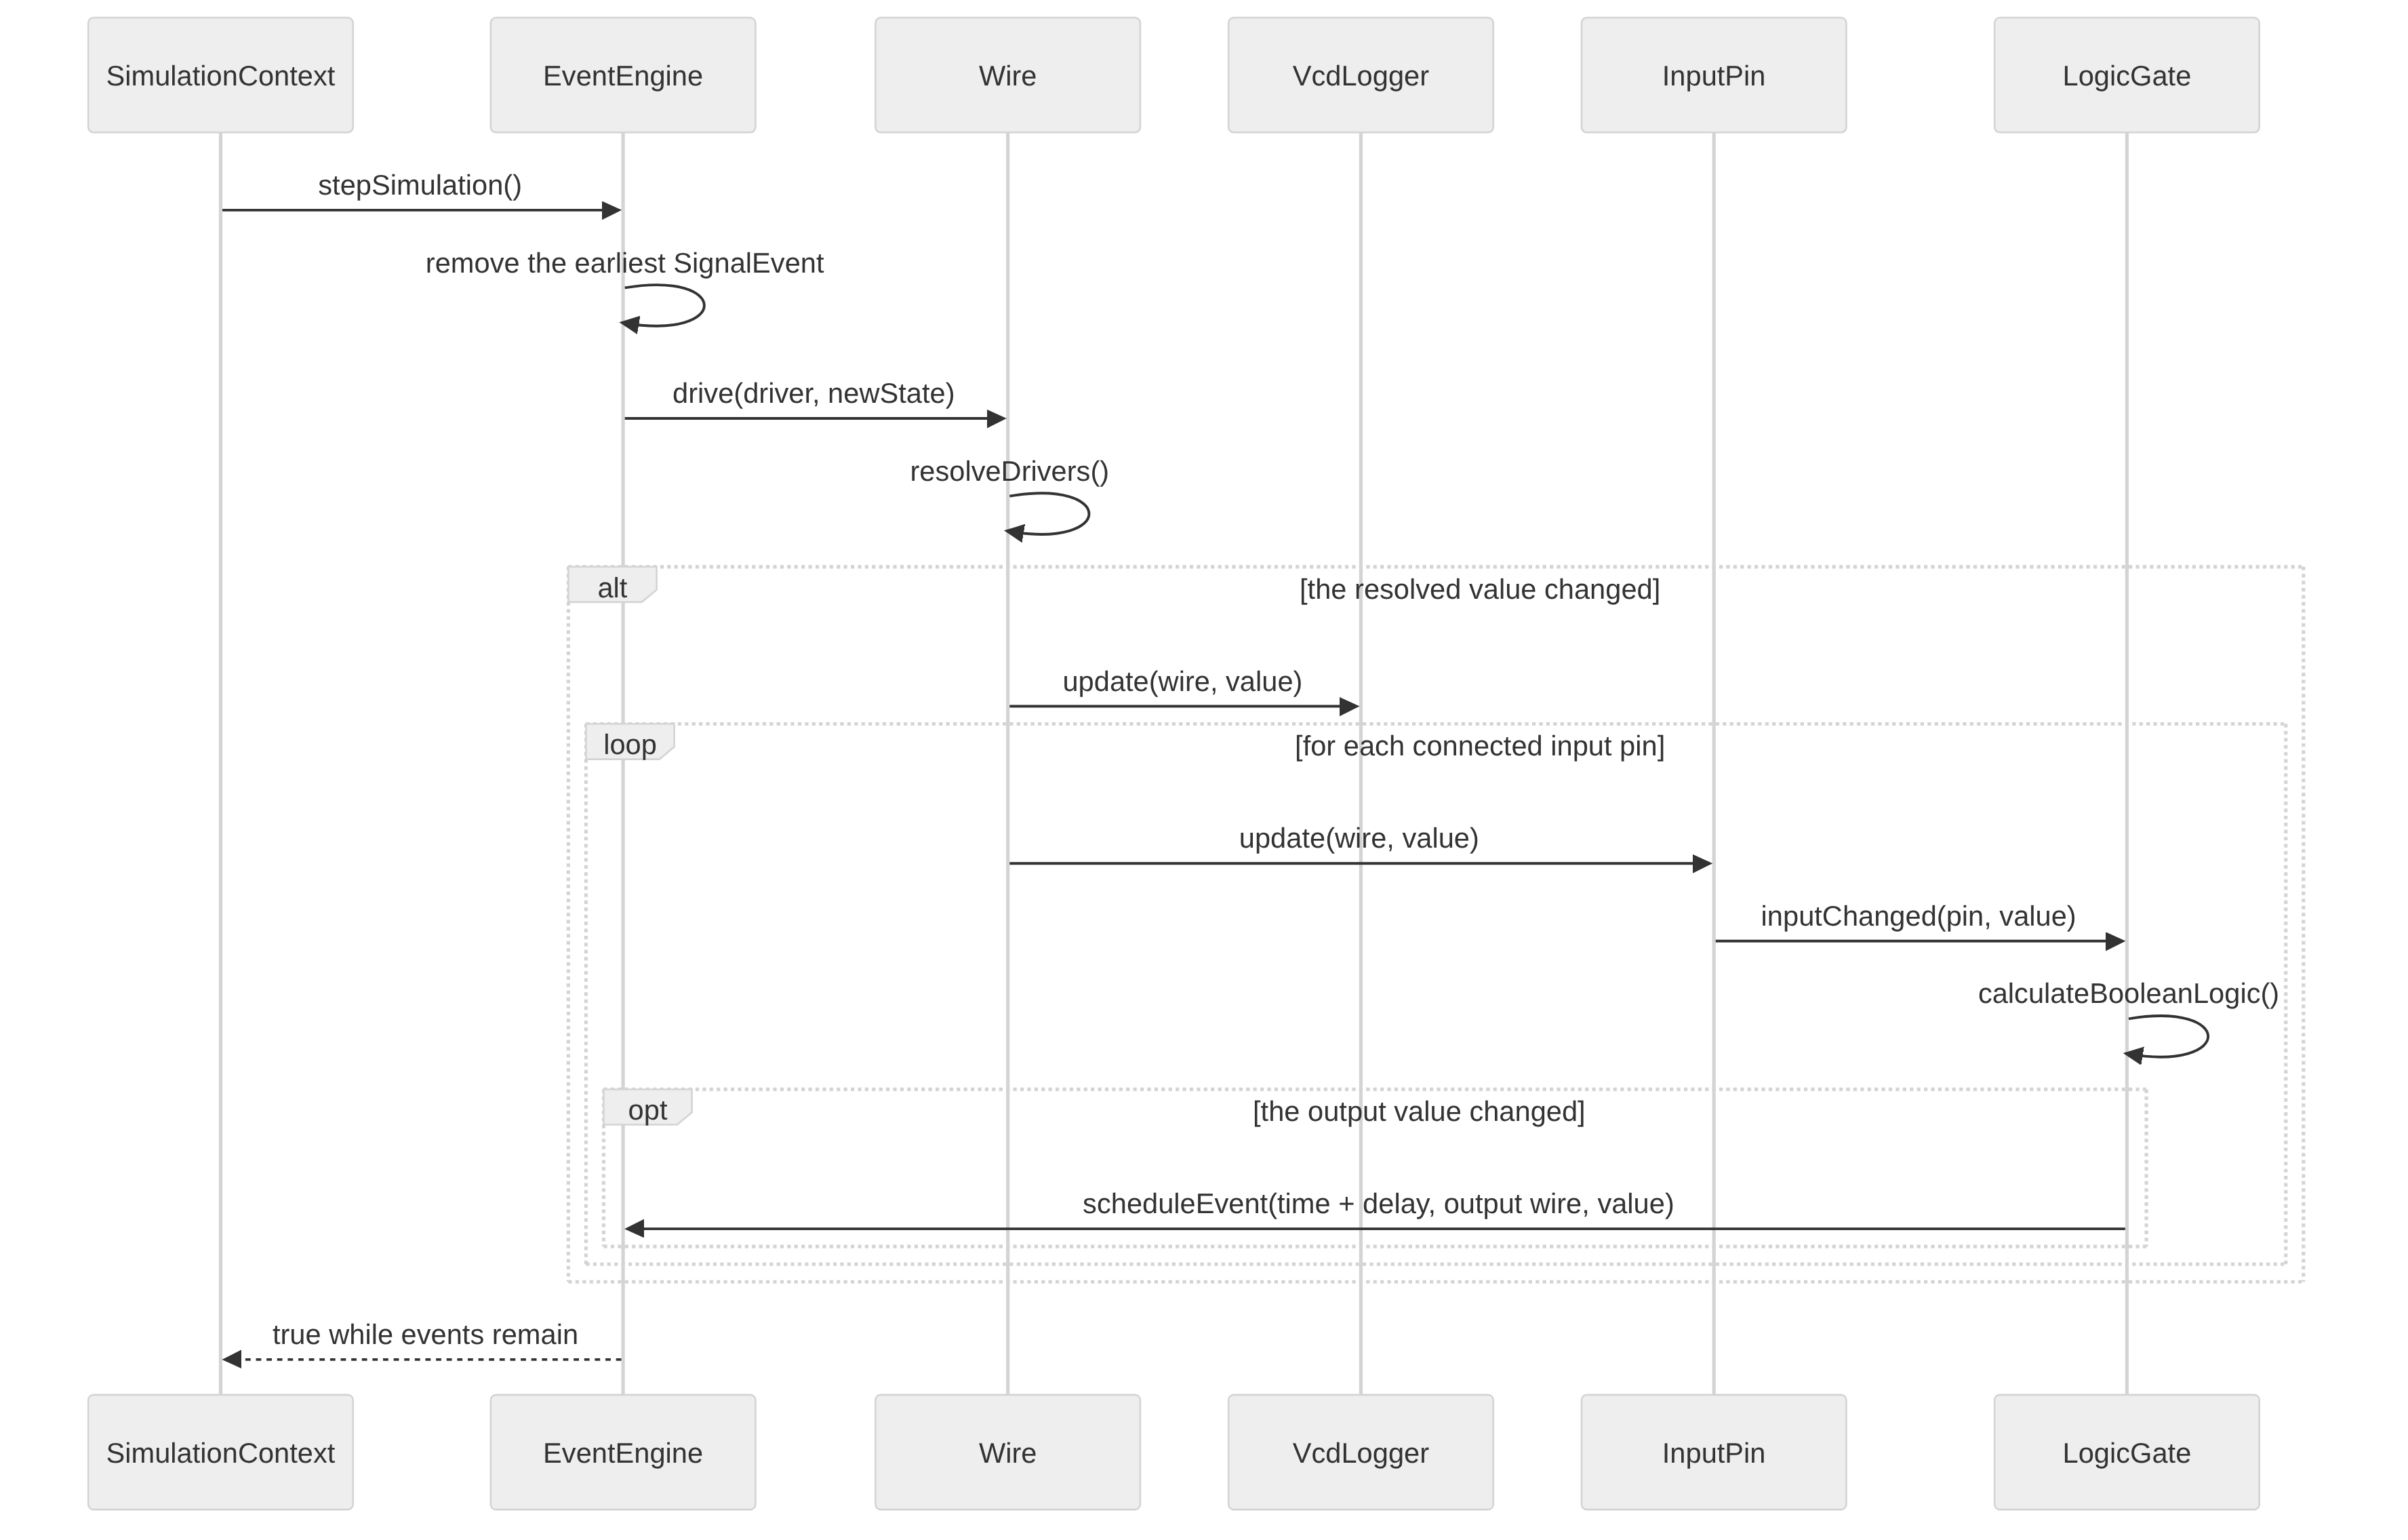
\includegraphics[width=\textwidth]{sequenceDiagramEvent.png}
\caption{Sequence diagram of the processing of one event}
\label{fig:seqevent}
\end{figure}

A wire resolves the values of its drivers on each update.
The wire takes the value X when one driver holds X or when two drivers disagree.
It takes the value Z when every driver has released it.
It takes the common value when the remaining drivers agree.
A stuck-at fault overrides all drivers until the end of the run.

\subsection{State Model}

Figure~\ref{fig:state} presents the states of a flip-flop.
A flip-flop starts in \texttt{LowState} and changes state only on a rising clock edge.
A data input of X or Z moves it to \texttt{UnknownState}, and the next known data value restores a known state.
The transitions that keep a flip-flop in its present state do not appear in the figure.

\begin{figure}[H]
\centering
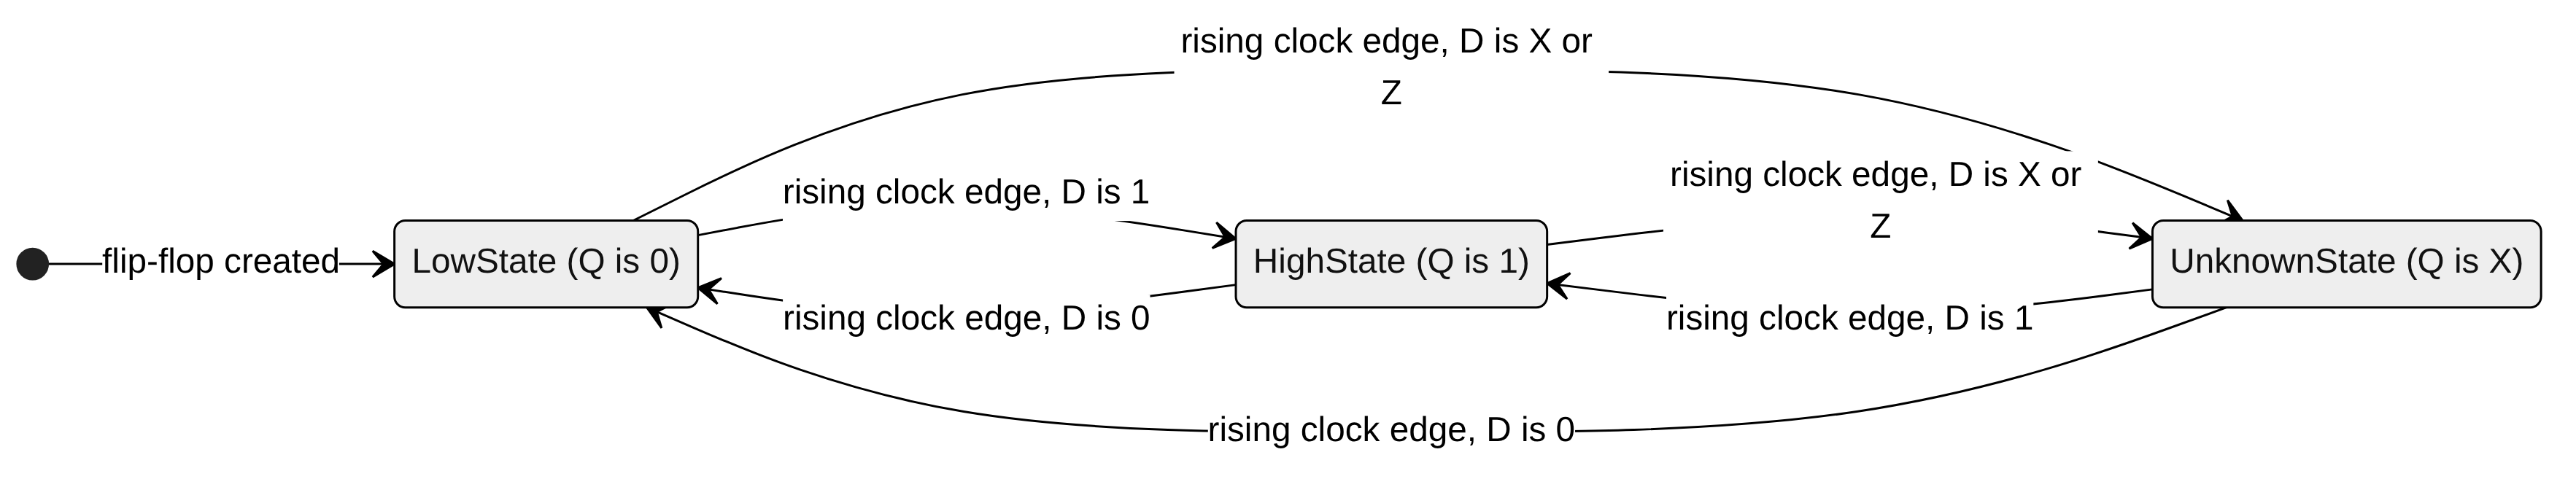
\includegraphics[width=\textwidth]{stateDiagramMemory.png}
\caption{State diagram of a flip-flop}
\label{fig:state}
\end{figure}

\subsection{Netlist Language}

A netlist is a plain text file with one command on each line.
Figure~\ref{fig:netlist} presents a half adder that uses the language.
The \texttt{SIM\_TIME} command sets the duration, and \texttt{WIRE} declares a wire.
Each gate line gives the gate type, a name, a delay in nanoseconds, the input wires, and the output wire.
\texttt{STIMULUS} sets an input at a given time, and \texttt{ASSERT} checks a wire at a given time.
The language also provides macros through \texttt{DEF} and \texttt{ENDDEF}, Boolean functions through \texttt{FUNC}, faults through \texttt{FAULT}, and a library of adders, multiplexers, and decoders.

\begin{figure}[H]
\centering
\begin{lstlisting}
# Half adder
SIM_TIME 100

WIRE A
WIRE B
WIRE Sum
WIRE Carry

XOR sum_gate 10 A B Sum
AND carry_gate 10 A B Carry

STIMULUS 0 A 1
STIMULUS 0 B 1

ASSERT 50 Sum 0
ASSERT 50 Carry 1
\end{lstlisting}
\caption{Netlist of a half adder with stimuli and assertions}
\label{fig:netlist}
\end{figure}

\subsection{Analysis Algorithms}

\textbf{Static timing analysis.}
The analyzer finds the slowest route through the components with a memoized depth-first search.
A route may start at a flip-flop, whose own delay represents its clock-to-output time, and it ends at the data input of the next flip-flop.
The maximum clock frequency is the inverse of the critical path delay.

\textbf{Truth tables and state tables.}
The generator builds a fresh circuit for each input combination, applies the inputs, and runs the simulation until no event remains.
For a sequential circuit, it also forces each combination of stored values and reads the next state from the data inputs of the flip-flops.
This table includes the internal variables, as the reference paper proposes for sequential circuits \refDezan{}.

\textbf{Equivalence checking.}
The checker generates the tables of two circuits and compares them row by row, following the method of the reference paper \refDezan{}.
It reports the first row that differs.

\textbf{Fault coverage.}
The analyzer simulates the circuit once without a fault.
It then repeats the simulation once for each wire stuck at 0 and once for each wire stuck at 1.
A fault counts as detected when an output or a flip-flop holds a known value that differs from the fault-free value at some time.

\textbf{Schematic layout.}
The layout places components in columns by signal flow, which follows the layered drawing method of Sugiyama, Tagawa, and Toda \refSugiyama{}.
It orders the components in each column to reduce wire crossings, and it routes wires through tracks between the columns.

\subsection{User Interfaces}

The desktop application, built with Java Swing, provides an editor beside tabs for the log, waveform, schematic, analysis, and user guide.
Figure~\ref{fig:desktop} presents the waveform tab with the two-bit counter from the sample set.
Figure~\ref{fig:schematic} presents the schematic tab with a two-bit adder built from macros.
The highlighted route in this figure is the critical path, and a time slider colors each wire by its value.

\begin{figure}[H]
\centering
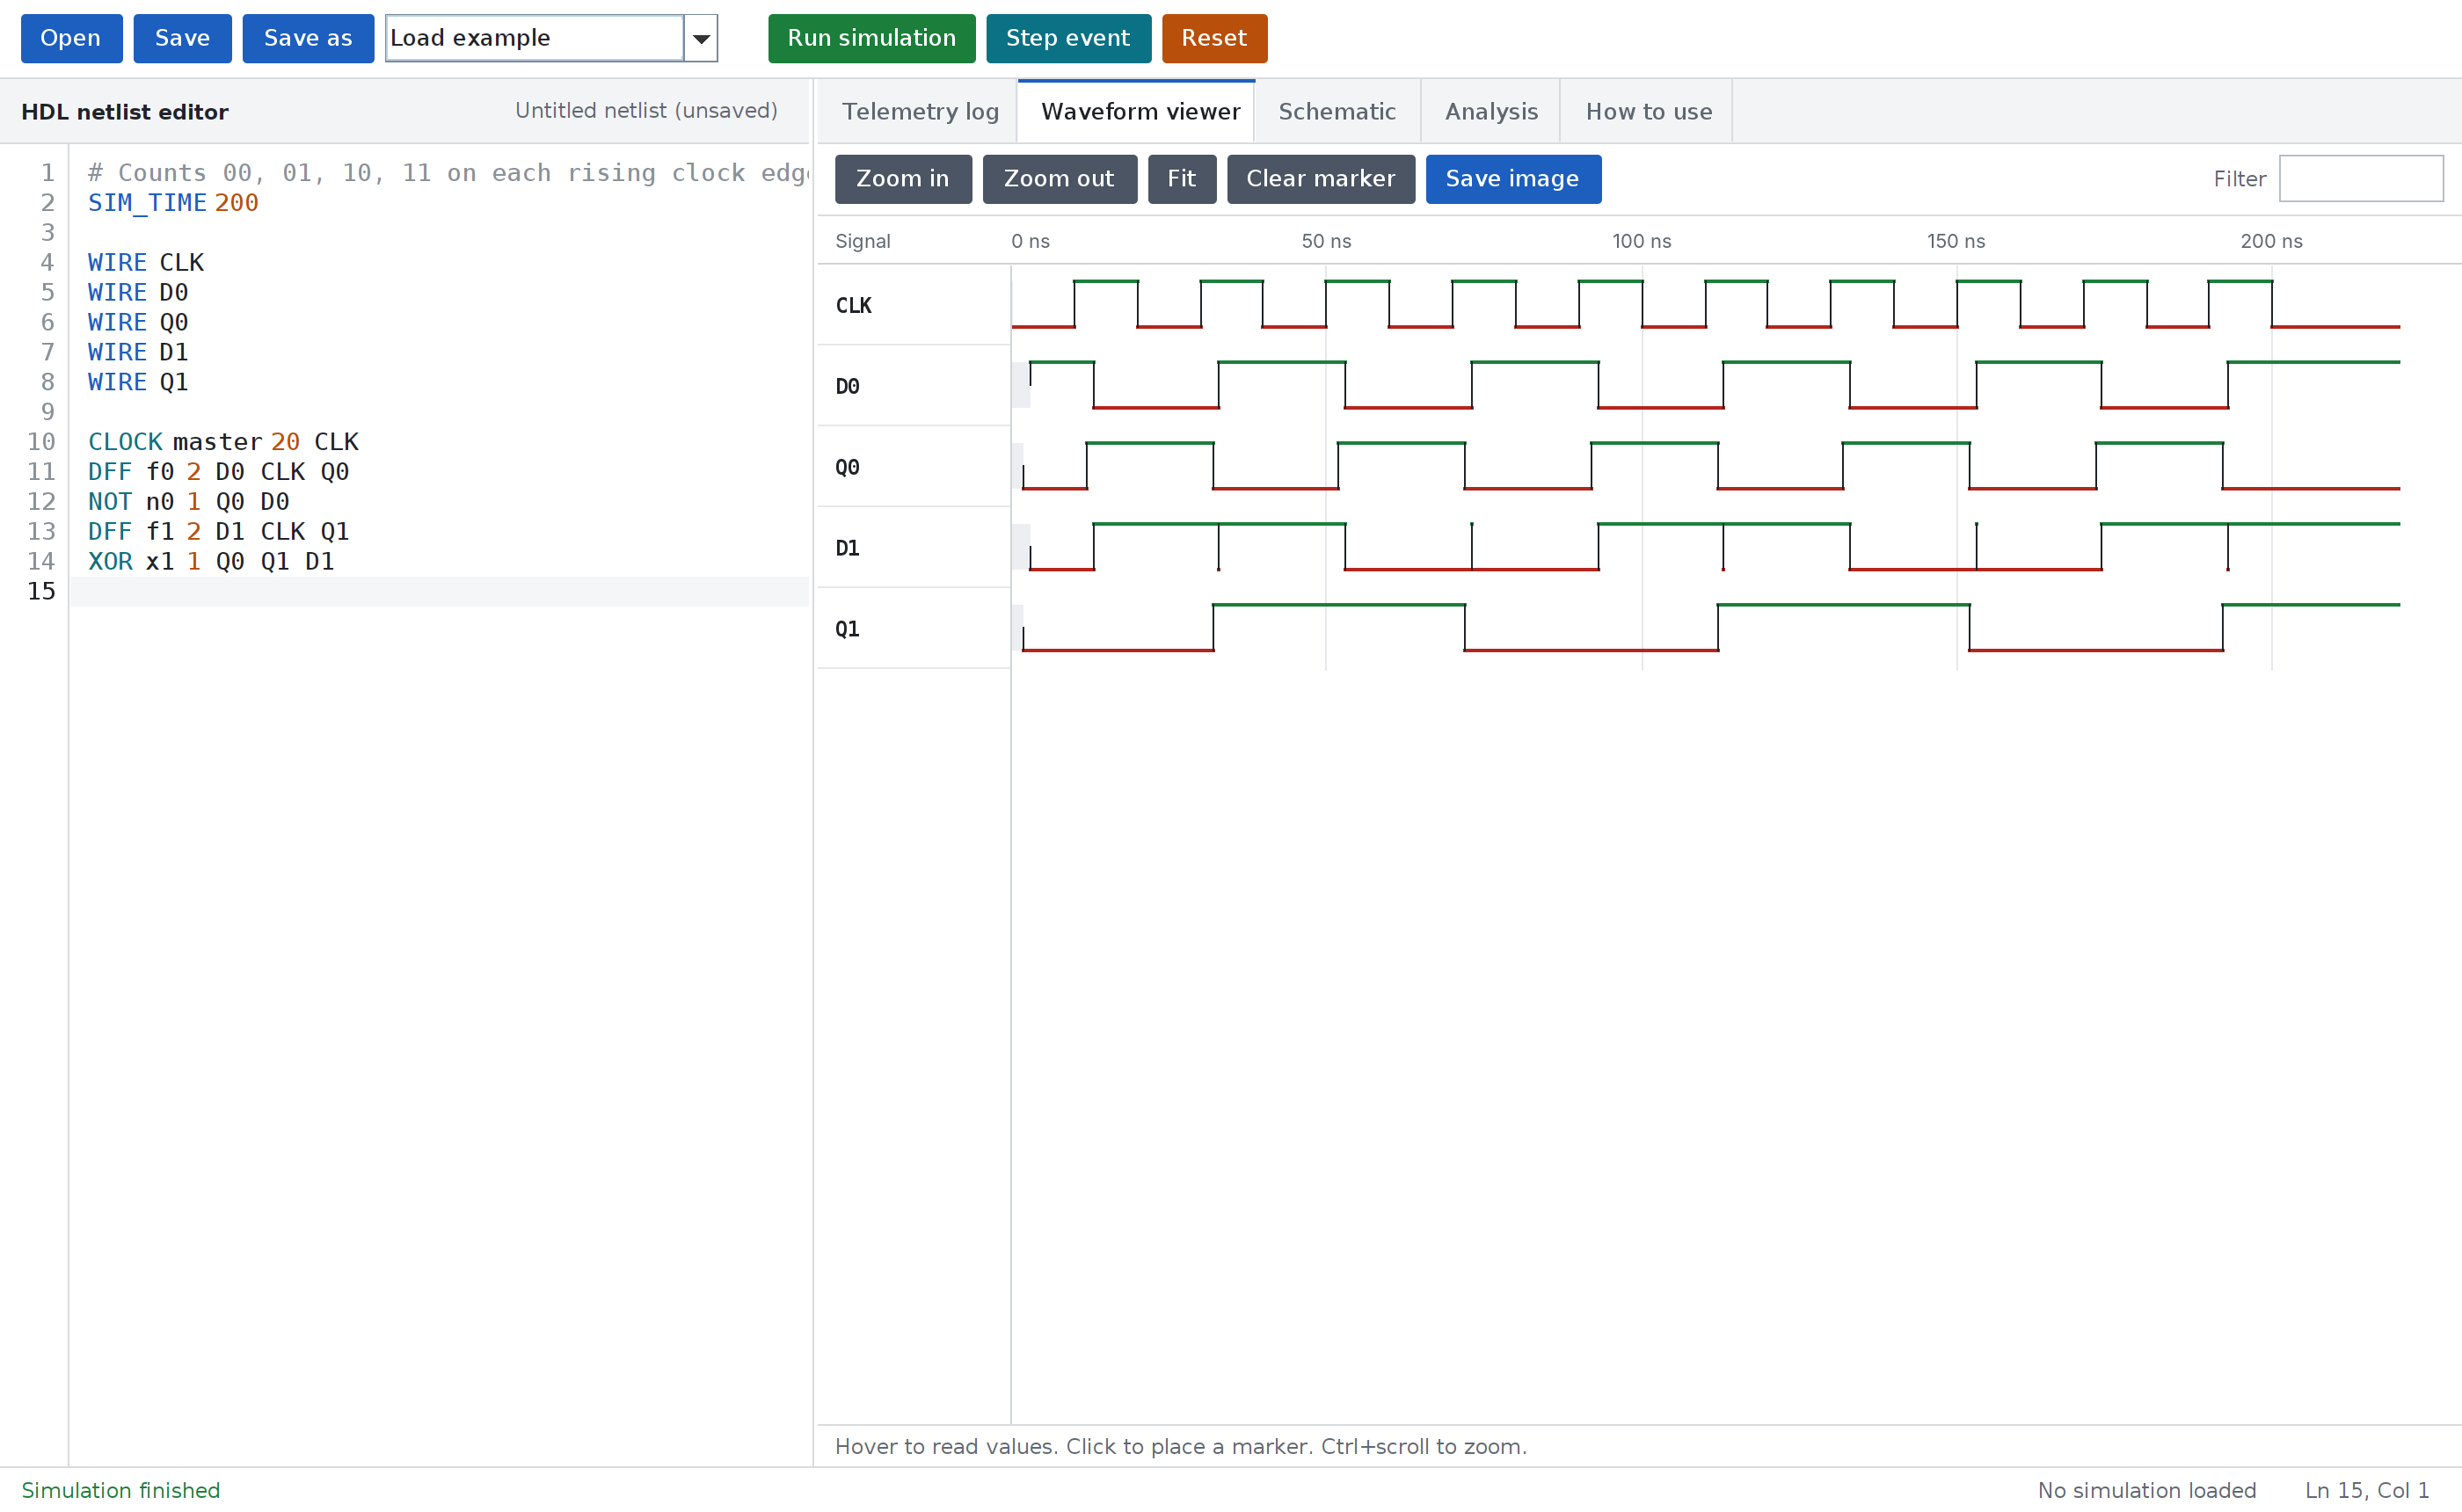
\includegraphics[width=\textwidth]{desktop-waveform.png}
\caption{Waveform tab of the desktop application}
\label{fig:desktop}
\end{figure}

\begin{figure}[H]
\centering
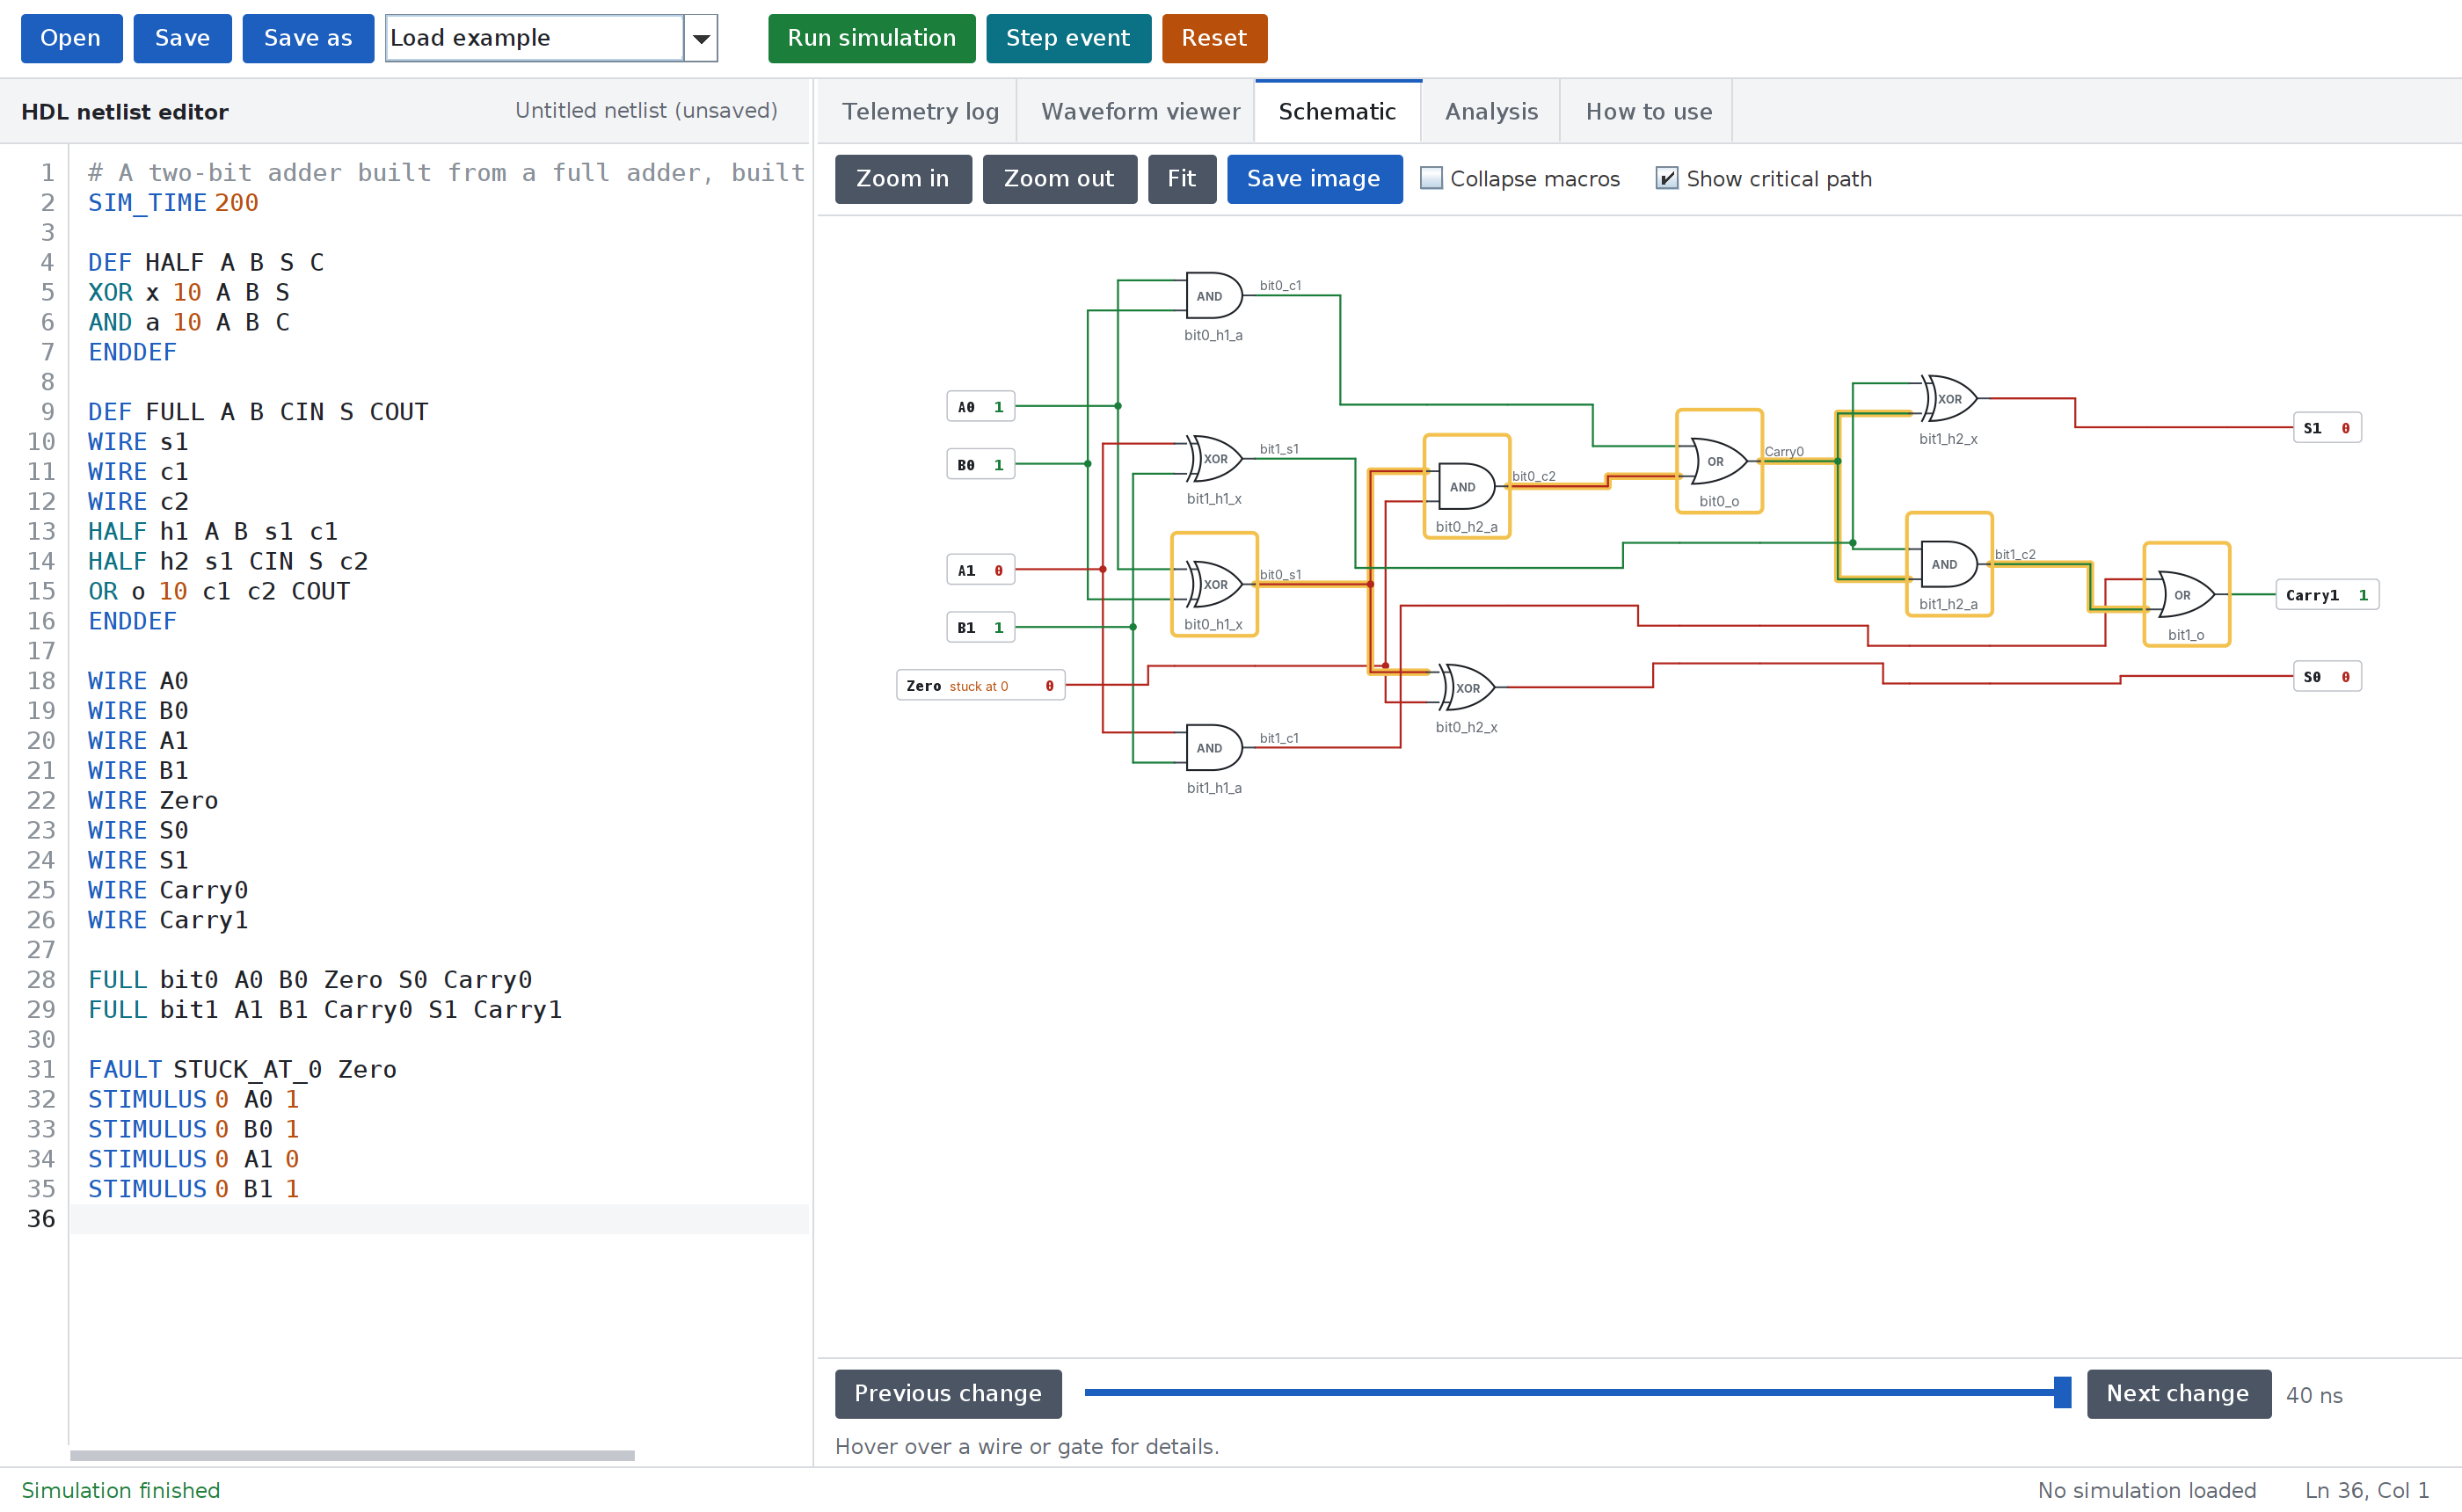
\includegraphics[width=\textwidth]{desktop-schematic.png}
\caption{Schematic tab with the critical path highlighted}
\label{fig:schematic}
\end{figure}

The hosted browser version \refHosted{} offers the same tabs and the same results.
The command line tool exposes each operation as a command with an exit status, so scripts can use it for automated checks.
Exported VCD files open in external viewers such as GTKWave \refGTKWave{}.
